\chapter{Analiza wybranych typów Malware}
\newpage
\section{Klasyczny Wirus} 
\begin{table}[htbp]
    \begin{tabular}{|c|m{10cm}|}
    \hline
    \textbf{Cecha} & \textbf{Opis}\\
    \hline
    \textbf{Ogólna zasada} & Działa na podobnych zasadach jak biologiczny wirus.\\
    \hline
    \textbf{Zależność} & Nie jest samodzielnym programem, potrzebuje „żywiciela” – dodaje swój kod do legalnych plików (np. programów, dokumentów).\\
    \hline
    \textbf{Powielanie} & Powiela się samodzielnie, po uruchomieniu zainfekowanego programu wirus się uruchamia i infekuje następne pliki.\\
    \hline
    \textbf{Zadanie} & Jego zadanie to najczęściej niszczenie i modyfikowanie plików lub uszkadzanie systemu operacyjnego.\cite{wirus}\\
    \hline
    \end{tabular}
    \caption{Charakterystyka wirusa komputerowego}
    \label{tab:Klasyczny wirus}
\end{table} 
\begin{figure}[!h]
    \centering
    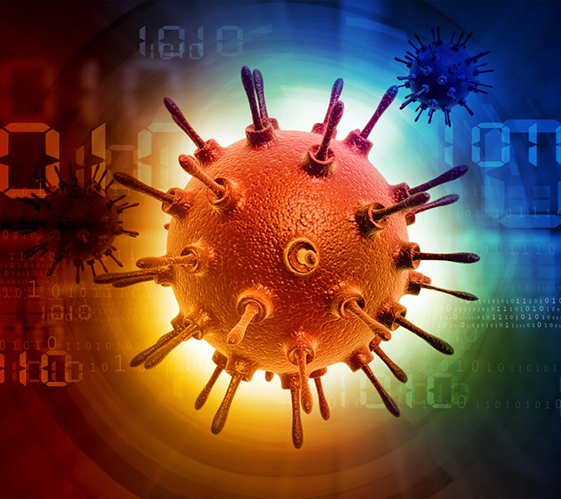
\includegraphics[width=1\linewidth]{wirus_rys.png}
    \caption{Artystyczna wizja wirusa komputerowego \cite{grafiki}}
    \label{wirus}
\end{figure}
\newpage
\subsection{Przykład - CIH ,,Czarnobyl'' \index{Czarnobyl}}
\begin{figure}[!h]
    \centering
    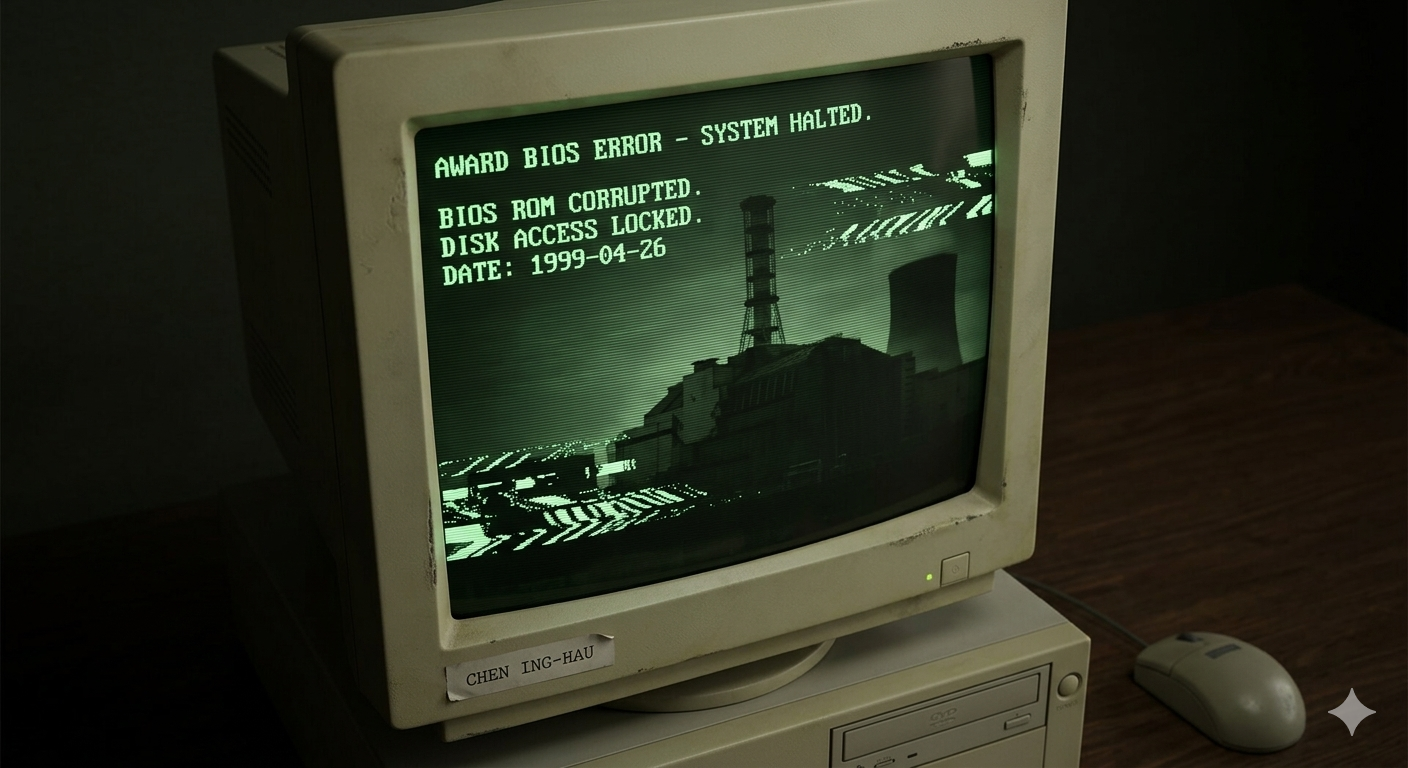
\includegraphics[width=1\linewidth]{czarnobyl.png}
    \caption{Wirus oczami \ac{AI} \cite{grafiki}}
    \label{fig:czarnobyl}
    \index{AI}
\end{figure}
\begin{itemize}
    \item \textbf{Pochodzenie i twórca:} Tajwański student {Chen Ing-Hau}
    \item \textbf{Data ataku:} {26 kwietnia 1999}
    \item \textbf{Metoda Kamuflażu:} {„Spacefiller”}
    \item \textbf{Skutki infekcji:} {Blokada dysku i atak na Bios}
    \item \textbf{Mity:} {Totalne zniszczenie płyty głównej} \cite{wirus_przyklad}
\end{itemize}
\newpage
\section{Robak}
Jaka zaznaczono wcześniej w Tabeli \ref{tab:Klasyczny wirus} na stronie \pageref{tab:Klasyczny wirus}, klasyczny wirus potrzebuje żywiciela. Robak\index{robak} działa zupełnie inaczej:
\begin{itemize}
    \item Jest w pełni samodzielnym programem
    \item Rozprzestrzenia się automatycznie i replikuje przez sieć, bez konieczności działania użytkownika.
    \item Jego głównym celem jest zużywanie zasobów sieciowych lub otwieranie „tylnych furtek” (\textit{backdoor}\index{backdoor}). \cite{robak}
\end{itemize}
\begin{figure}[!h]
    \centering
    \includegraphics[width=1\linewidth]{robak.png}
    \caption{Symboliczna reprezentacja robaka komputerowego przełamującego zabezpieczenia systemu. \cite{grafiki}}
    \label{fig:robak}
\end{figure}
\subsection{Matematyczny model\index{model matematyczny} infekcji}
\begin{equation}
    I(t) = I_0 \cdot e^{rt}
    \label{eq:infekcja}
\end{equation}
Jak wynika ze wzoru \eqref{eq:infekcja}, w którym $I_0$ to początkowa liczba zainfekowanych maszyn, a $r$ to wskaźnik infekcji, liczba zarażonych komputerów rośnie lawinowo w bardzo krótkim czasie. 
\newpage
\subsection{Przykład – Robak Morrisa\index{Robak Morrisa}}
\begin{figure}[!h]
    \centering
    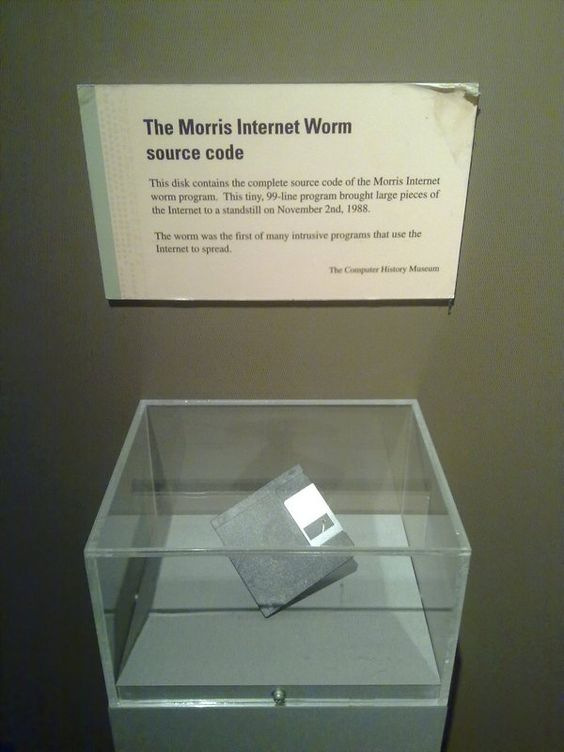
\includegraphics[width=0.5\linewidth]{robak_muzeum.png}
    \caption{Dyskietka z kodem źródłowym w muzeum. \cite{grafiki}}
    \label{fig:robak_muzeum}
\end{figure}
\begin{itemize}
    \item \textbf{Pochodzenie i twórca} Amerykański student Robert Tappan Morris.
    \item \textbf{Data ataku:} 2 listopada 1988 r.
    \item \textbf{Cel:} Niegroźne badanie luk w zabezpieczeniach
    \item \textbf{Skutki infekcji:} Paraliż około 10\% ówczesnego Internetu (ponad 6 tys. komputerów)
    \item \textbf{Konsekwencje dla autora:} Wyrok sądowy \cite{robak_morris}
\end{itemize}
\newpage